\documentclass{standalone}
\usepackage{tikz}
\usetikzlibrary{patterns, positioning}


\begin{document}
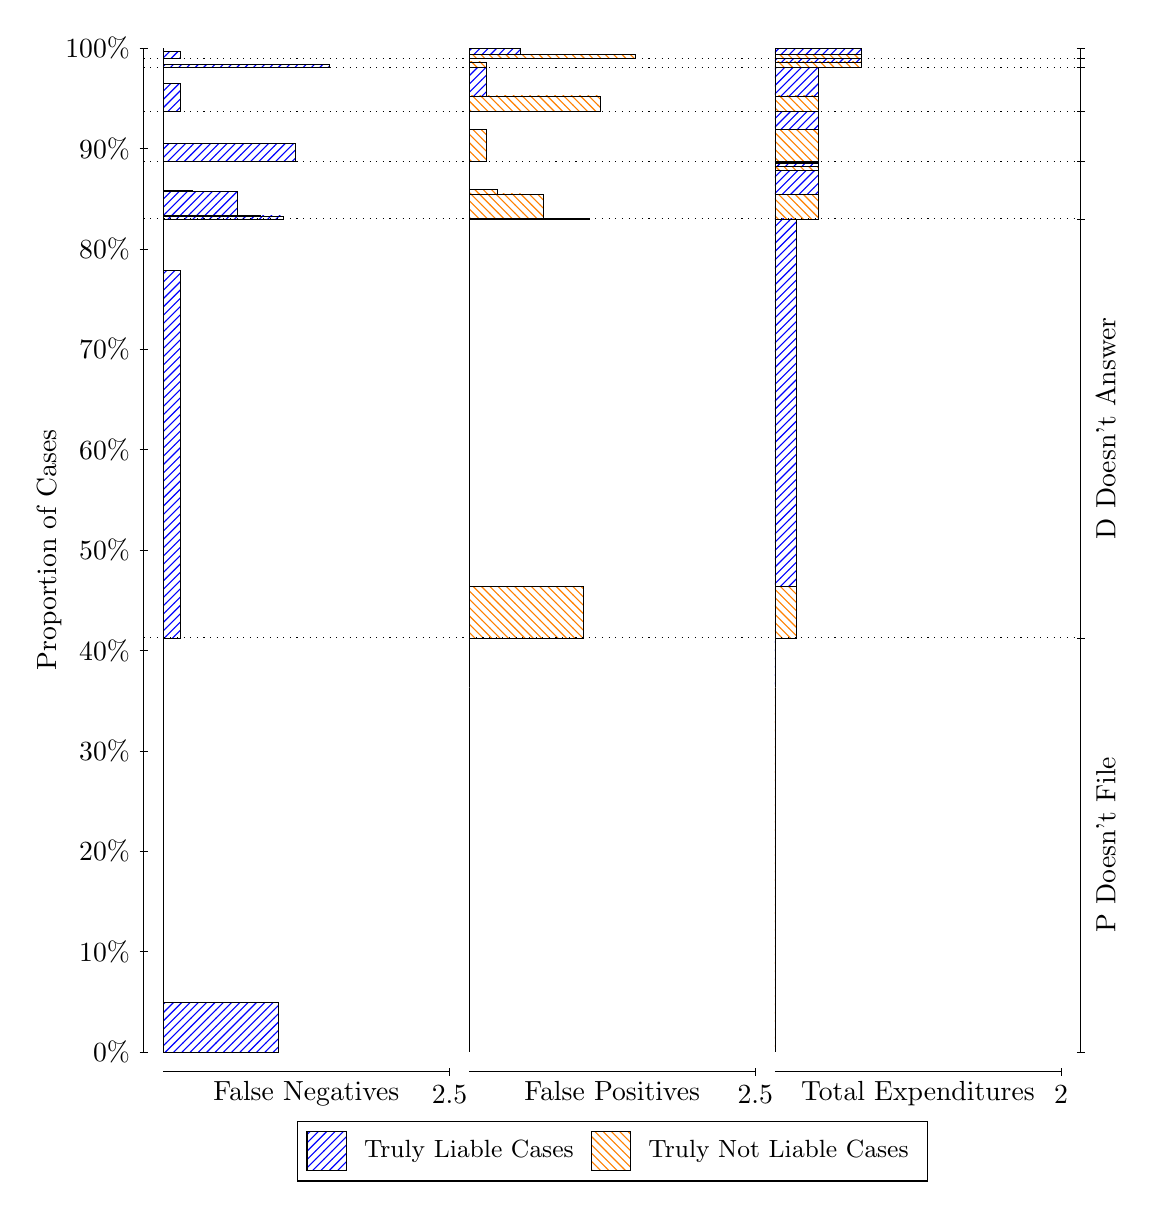
\begin{tikzpicture}
\draw[black, very thin] (1.5,1.75) -- (1.5,14.5);
\node[rotate=90, text=black, anchor=center] at (0.3, 8.125) {Proportion of Cases};
\draw[black, very thin] (1.45,1.75) -- (1.55,1.75);
\node[text=black, anchor=east] at (1.45, 1.75) {0\%};
\draw[black, very thin] (1.45,3.025) -- (1.55,3.025);
\node[text=black, anchor=east] at (1.45, 3.025) {10\%};
\draw[black, very thin] (1.45,4.3) -- (1.55,4.3);
\node[text=black, anchor=east] at (1.45, 4.3) {20\%};
\draw[black, very thin] (1.45,5.575) -- (1.55,5.575);
\node[text=black, anchor=east] at (1.45, 5.575) {30\%};
\draw[black, very thin] (1.45,6.85) -- (1.55,6.85);
\node[text=black, anchor=east] at (1.45, 6.85) {40\%};
\draw[black, very thin] (1.45,8.125) -- (1.55,8.125);
\node[text=black, anchor=east] at (1.45, 8.125) {50\%};
\draw[black, very thin] (1.45,9.4) -- (1.55,9.4);
\node[text=black, anchor=east] at (1.45, 9.4) {60\%};
\draw[black, very thin] (1.45,10.675) -- (1.55,10.675);
\node[text=black, anchor=east] at (1.45, 10.675) {70\%};
\draw[black, very thin] (1.45,11.95) -- (1.55,11.95);
\node[text=black, anchor=east] at (1.45, 11.95) {80\%};
\draw[black, very thin] (1.45,13.225) -- (1.55,13.225);
\node[text=black, anchor=east] at (1.45, 13.225) {90\%};
\draw[black, very thin] (1.45,14.5) -- (1.55,14.5);
\node[text=black, anchor=east] at (1.45, 14.5) {100\%};

\draw[black, very thin] (13.4,1.75) -- (13.4,14.5);
\draw[black, very thin] (13.35,1.75) -- (13.45,1.75);
\node[anchor=west] at (13.35, 1.75) {};
\draw[black, very thin] (13.35,7.01) -- (13.45,7.01);
\node[anchor=west] at (13.35, 7.01) {};
\draw[black, very thin] (13.35,12.33) -- (13.45,12.33);
\node[anchor=west] at (13.35, 12.33) {};
\draw[black, very thin] (13.35,13.06) -- (13.45,13.06);
\node[anchor=west] at (13.35, 13.06) {};
\draw[black, very thin] (13.35,13.696) -- (13.45,13.696);
\node[anchor=west] at (13.35, 13.696) {};
\draw[black, very thin] (13.35,14.251) -- (13.45,14.251);
\node[anchor=west] at (13.35, 14.251) {};
\draw[black, very thin] (13.35,14.369) -- (13.45,14.369);
\node[anchor=west] at (13.35, 14.369) {};
\draw[black, very thin] (13.35,14.5) -- (13.45,14.5);
\node[anchor=west] at (13.35, 14.5) {};

\draw[black, very thin, pattern color=blue, pattern=north east lines] (1.75,1.75) rectangle (3.2033,2.3828);
\draw[black, very thin, pattern color=orange, pattern=north west lines] (1.75,2.3828) rectangle (1.75,7.01);
\draw[black, very thin, pattern color=blue, pattern=north east lines] (1.75,7.01) rectangle (1.968,11.675);
\draw[black, very thin, pattern color=orange, pattern=north west lines] (1.75,11.675) rectangle (1.75,12.33);
\draw[black, very thin, pattern color=blue, pattern=north east lines] (1.75,12.33) rectangle (3.276,12.368);
\draw[black, very thin, pattern color=blue, pattern=north east lines] (1.75,12.368) rectangle (2.9853,12.379);
\draw[black, very thin, pattern color=blue, pattern=north east lines] (1.75,12.379) rectangle (2.6947,12.676);
\draw[black, very thin, pattern color=blue, pattern=north east lines] (1.75,12.676) rectangle (2.404,12.681);
\draw[black, very thin, pattern color=blue, pattern=north east lines] (1.75,12.681) rectangle (2.1133,12.688);
\draw[black, very thin, pattern color=orange, pattern=north west lines] (1.75,12.688) rectangle (1.75,13.06);
\draw[black, very thin, pattern color=blue, pattern=north east lines] (1.75,13.06) rectangle (3.4213,13.293);
\draw[black, very thin, pattern color=orange, pattern=north west lines] (1.75,13.293) rectangle (1.75,13.696);
\draw[black, very thin, pattern color=blue, pattern=north east lines] (1.75,13.696) rectangle (1.968,14.053);
\draw[black, very thin, pattern color=orange, pattern=north west lines] (1.75,14.053) rectangle (1.75,14.251);
\draw[black, very thin, pattern color=blue, pattern=north east lines] (1.75,14.251) rectangle (3.8573,14.295);
\draw[black, very thin, pattern color=orange, pattern=north west lines] (1.75,14.295) rectangle (1.75,14.369);
\draw[black, very thin, pattern color=blue, pattern=north east lines] (1.75,14.369) rectangle (1.968,14.454);
\draw[black, very thin, pattern color=orange, pattern=north west lines] (1.75,14.454) rectangle (1.75,14.5);
\draw[black, very thin, pattern color=orange, pattern=north west lines] (5.6333,1.75) rectangle (5.6333,6.3773);
\draw[black, very thin, pattern color=blue, pattern=north east lines] (5.6333,6.3773) rectangle (5.6333,7.01);
\draw[black, very thin, pattern color=orange, pattern=north west lines] (5.6333,7.01) rectangle (7.0867,7.6652);
\draw[black, very thin, pattern color=blue, pattern=north east lines] (5.6333,7.6652) rectangle (5.6333,12.33);
\draw[black, very thin, pattern color=orange, pattern=north west lines] (5.6333,12.33) rectangle (7.1593,12.334);
\draw[black, very thin, pattern color=orange, pattern=north west lines] (5.6333,12.334) rectangle (6.8687,12.34);
\draw[black, very thin, pattern color=orange, pattern=north west lines] (5.6333,12.34) rectangle (6.578,12.637);
\draw[black, very thin, pattern color=orange, pattern=north west lines] (5.6333,12.637) rectangle (6.2873,12.648);
\draw[black, very thin, pattern color=orange, pattern=north west lines] (5.6333,12.648) rectangle (5.9967,12.702);
\draw[black, very thin, pattern color=blue, pattern=north east lines] (5.6333,12.702) rectangle (5.706,12.709);
\draw[black, very thin, pattern color=blue, pattern=north east lines] (5.6333,12.709) rectangle (5.6333,13.06);
\draw[black, very thin, pattern color=orange, pattern=north west lines] (5.6333,13.06) rectangle (5.8513,13.463);
\draw[black, very thin, pattern color=blue, pattern=north east lines] (5.6333,13.463) rectangle (5.6333,13.696);
\draw[black, very thin, pattern color=orange, pattern=north west lines] (5.6333,13.696) rectangle (7.3047,13.893);
\draw[black, very thin, pattern color=blue, pattern=north east lines] (5.6333,13.893) rectangle (5.8513,14.251);
\draw[black, very thin, pattern color=orange, pattern=north west lines] (5.6333,14.251) rectangle (5.8513,14.325);
\draw[black, very thin, pattern color=blue, pattern=north east lines] (5.6333,14.325) rectangle (5.6333,14.369);
\draw[black, very thin, pattern color=orange, pattern=north west lines] (5.6333,14.369) rectangle (7.7407,14.415);
\draw[black, very thin, pattern color=blue, pattern=north east lines] (5.6333,14.415) rectangle (6.2873,14.5);
\draw[black, very thin, pattern color=orange, pattern=north west lines] (9.5167,1.75) rectangle (9.5167,6.3773);
\draw[black, very thin, pattern color=blue, pattern=north east lines] (9.5167,6.3773) rectangle (9.5167,7.01);
\draw[black, very thin, pattern color=orange, pattern=north west lines] (9.5167,7.01) rectangle (9.7892,7.6652);
\draw[black, very thin, pattern color=blue, pattern=north east lines] (9.5167,7.6652) rectangle (9.7892,12.33);
\draw[black, very thin, pattern color=orange, pattern=north west lines] (9.5167,12.33) rectangle (10.062,12.637);
\draw[black, very thin, pattern color=blue, pattern=north east lines] (9.5167,12.637) rectangle (10.062,12.947);
\draw[black, very thin, pattern color=orange, pattern=north west lines] (9.5167,12.947) rectangle (10.062,13.001);
\draw[black, very thin, pattern color=blue, pattern=north east lines] (9.5167,13.001) rectangle (10.062,13.038);
\draw[black, very thin, pattern color=orange, pattern=north west lines] (9.5167,13.038) rectangle (10.062,13.049);
\draw[black, very thin, pattern color=blue, pattern=north east lines] (9.5167,13.049) rectangle (10.062,13.06);
\draw[black, very thin, pattern color=orange, pattern=north west lines] (9.5167,13.06) rectangle (10.062,13.463);
\draw[black, very thin, pattern color=blue, pattern=north east lines] (9.5167,13.463) rectangle (10.062,13.696);
\draw[black, very thin, pattern color=orange, pattern=north west lines] (9.5167,13.696) rectangle (10.062,13.893);
\draw[black, very thin, pattern color=blue, pattern=north east lines] (9.5167,13.893) rectangle (10.062,14.251);
\draw[black, very thin, pattern color=orange, pattern=north west lines] (9.5167,14.251) rectangle (10.607,14.325);
\draw[black, very thin, pattern color=blue, pattern=north east lines] (9.5167,14.325) rectangle (10.607,14.369);
\draw[black, very thin, pattern color=orange, pattern=north west lines] (9.5167,14.369) rectangle (10.607,14.415);
\draw[black, very thin, pattern color=blue, pattern=north east lines] (9.5167,14.415) rectangle (10.607,14.5);
\draw[black, dotted] (1.5,7.01) -- (13.4,7.01);
\draw[black, dotted] (1.5,12.33) -- (13.4,12.33);
\draw[black, dotted] (1.5,13.06) -- (13.4,13.06);
\draw[black, dotted] (1.5,13.696) -- (13.4,13.696);
\draw[black, dotted] (1.5,14.251) -- (13.4,14.251);
\draw[black, dotted] (1.5,14.369) -- (13.4,14.369);
\draw[black, very thin] (1.75,1.5) -- (5.3833,1.5);
\node[text=black, anchor=north] at (3.5667, 1.5) {False Negatives};
\draw[black, very thin] (5.3833,1.45) -- (5.3833,1.55);
\node[text=black, anchor=north] at (5.3833, 1.45) {2.5};

\draw[black, very thin] (5.6333,1.5) -- (9.2667,1.5);
\node[text=black, anchor=north] at (7.45, 1.5) {False Positives};
\draw[black, very thin] (9.2667,1.45) -- (9.2667,1.55);
\node[text=black, anchor=north] at (9.2667, 1.45) {2.5};

\draw[black, very thin] (9.5167,1.5) -- (13.15,1.5);
\node[text=black, anchor=north] at (11.333, 1.5) {Total Expenditures};
\draw[black, very thin] (13.15,1.45) -- (13.15,1.55);
\node[text=black, anchor=north] at (13.15, 1.45) {2};

\node[text=black, centered, rotate=90] at (13.72, 4.38) {P Doesn't File};
\node[text=black, centered, rotate=90] at (13.72, 9.6702) {D Doesn't Answer};






\draw (7.449999999999999,1.5) node[draw=none] (baseCoordinate) {};
\begin{scope}[align=center]
        \matrix[scale=0.5, draw=black, below=0.5cm of baseCoordinate, nodes={draw}, column sep=0.1cm]{
            \node[rectangle, draw, minimum width=0.5cm, minimum height=0.5cm, pattern color=blue, pattern=north east lines] {}; &
            \node[draw=none, font=\small, text=black] (B) {Truly Liable Cases}; &
            \node[rectangle, draw, minimum width=0.5cm, minimum height=0.5cm, pattern color=orange, pattern=north west lines] {}; &
            \node[draw=none, font=\small, text=black] (B) {Truly Not Liable Cases}; \\
            };
\end{scope}

\end{tikzpicture}
\end{document}